In this chapter we will describe the design of neural network that will be able to process thermal images and decide what object they contain.
Workflow that we will follow will largely be a combination of workflows presented in Figures \ref{ml_workflow} and \ref{micro_workflow}.

We will first set concrete objectives, which will dictate what exactly we want to accomplish, while keeping in consideration various constraints.
We will then explore the dataset provided by Arribada Initiative, analyze different class representations and decide if it is appropriate for accomplishing objectives that we set earlier.

After dataset exploration we had to setup our development environment.
As software for creating and training ML models consists of many components and dependencies it is important to start with something that we know it works.
We will describe our AWS server setup, how we moved image data on it and why we decided to use Python Notebooks for algorithm development.

Image preparation was important step before model creation, as wanted to keep track of various metadata labels that were assigned to each image.
This involved parsing a large excel table and connecting images with correct labels.
Image preprocessing such as mean normalization and augmentation was then done.
We then designed and trained few CNN models with varying complexities and observed how well they behave on thermal image dataset.
We then optimized models with TFLite tools and compared accuracies and model sizes.
Models were then converted into a C char array format, ready to be tested on a actual microcontroller.

We will finish this chapter by describing the same workflow, but by using tools that Edge Impulse provides to the point where we will have our model ready to run on a microcontroller.
Using Edge Impulse will generally require less knowledge, less time and will lead to better results when compared to our setup.


\section{ Objectives}

The accuracy of our early detection system should be equal or similar to the one of human observer, no matter if we are operating in the daytime or nighttime.
Although our system will be placed on the paths that are regularly traversed by elephants, this does not mean that they will be only possible object on a image taken by a thermal camera.
Humans and various livestock, such as goats and cows, could also be photographed.
This means that we want to avoid reporting false positives, which means that our system should not incorrectly label a human or a livestock animal as an elephant.
At the same time we want avoid false negatives, where an elephant could pass by our system undetected.
These kind of mistakes could undermine the community's confidence of our early detection system and defeat our purpose.
This means that besides elephant detection, we should also focus on correctly labeling humans and livestock, while also providing a nature/random class for all other unexpected objects or simply images of nature.

It would be beneficial if thermal camera can take several pictures of the same object, thus increasing the confidence of computed label of the object.
However this is constrained by the image processing time and camera's field of view.
Thermal camera FLIR Lepton has a horizontal field of view of 57 degrees.
The closer elephant passes by the thermal camera the quicker he will traverse the camera's field of view, thus giving the camera less time for capture.
This problem can be solved by optimizing the execution time of the ML model or by placing the early detection system on far enough position from expected elephant's path.
As latter option might not be always possible, we should strive to keep the whole image processing time as short as possible.

Finally, as our neural network will be deployed on a microcontroller and not on a computer or a server we have to keep it simple and small.
Extra model complexity that might bring us few percents of accuracy will not matter much, if our model would be too large to fit on a microcontroller or too slow to run.


To summarize:
\begin{itemize}
    \item We will create an image classification ML model that will be capable of processing a thermal image and sorting it into one of possible 4 categories: elephant, human, cows and nature/random.
    \item Total image processing time should be as short as possible, we should try to keep it under 2 seconds.
    \item Model should be small enough to fit on a microcontroller of our choice, while still leaving some space for application code. Microcontroller of our choice (STM32F767) has 2 MB of flash memory so model size should be smaller than that.
\end{itemize}


\section{ Exploring the dataset} \label{exploring_dataset}

As mentioned in section \ref{arribada_init} thermal image dataset was provided by Arribada Initiative\cite{wildlabs-winners}\cite{arribada-assam}.
Images in dataset came from two different locations: Assam, India and ZSL Whipsnade Zoo, United Kingdom.

Assam served as a testing ground.
Arribada team positioned two camera traps on two locations that overlook paths commonly used by elephants.
Cameras were built otu from Raspberry Pi, PIR sensor, FLIR Lepton 2.5 camera and batteries, all of which were enclosed in a plastic housing.
Insides of the camera and an example of deployed camera can be seen on Figure \ref{assam_camera}.

\begin{figure}[ht]
    \begin{subfigure}{0.5\textwidth}
        \centering
        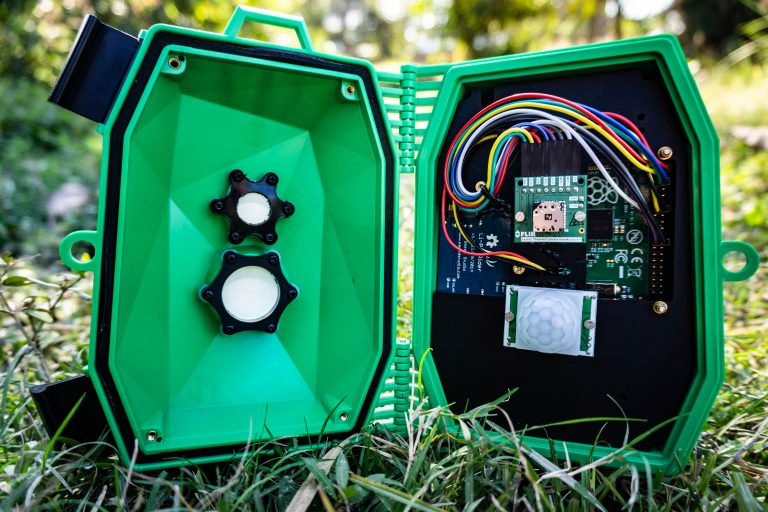
\includegraphics[width=1.0\linewidth, height=5cm]{assam_camera1.jpg} 
    \end{subfigure}
    \begin{subfigure}{0.5\textwidth}
        \centering
        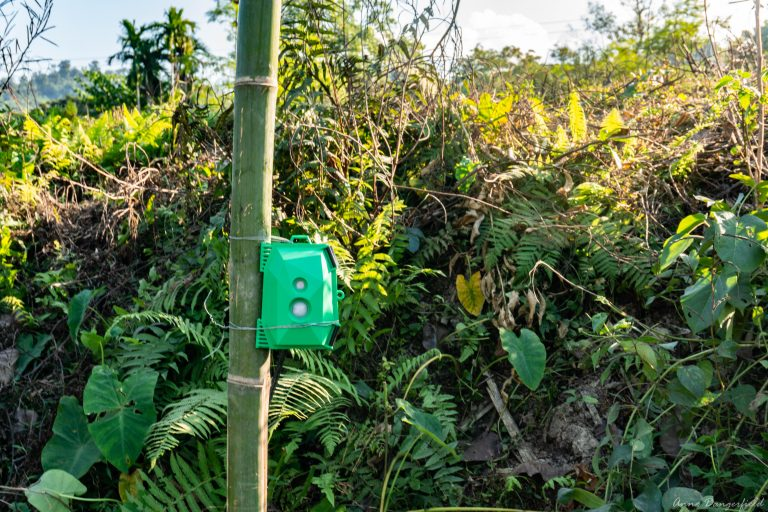
\includegraphics[width=1.0\linewidth, height=5cm]{assam_camera2.jpg}
    \end{subfigure}
    \caption{Camera trap used in Assam, India. Image source: Arribada Initiative \cite{arribada-assam}}
    \label{assam_camera}
\end{figure}

PIR sensor functioned as photo trigger, whenever an object passed in front of it camera made a picture.
This setup provided Arribada with elephant images in real life scenarios, however they could not capture elephants in variety of different conditions, such as different angles and distances.

This was accomplished in ZSL Whipsnade Zoo, where they could take many images of elephants in variety different conditions\cite{dataset_collection}.
PIR sensor trigger approach was dropped in favor of a 5 second time lapse trigger.
Two cameras were used again, however one of them now used FLIR Lepton 3.5, with better resolution.

Images of elephants that came from both locations can be seen on Figure \ref{four_elephants}.

\begin{figure}[ht]
    \centering
    \scalebox{.35}{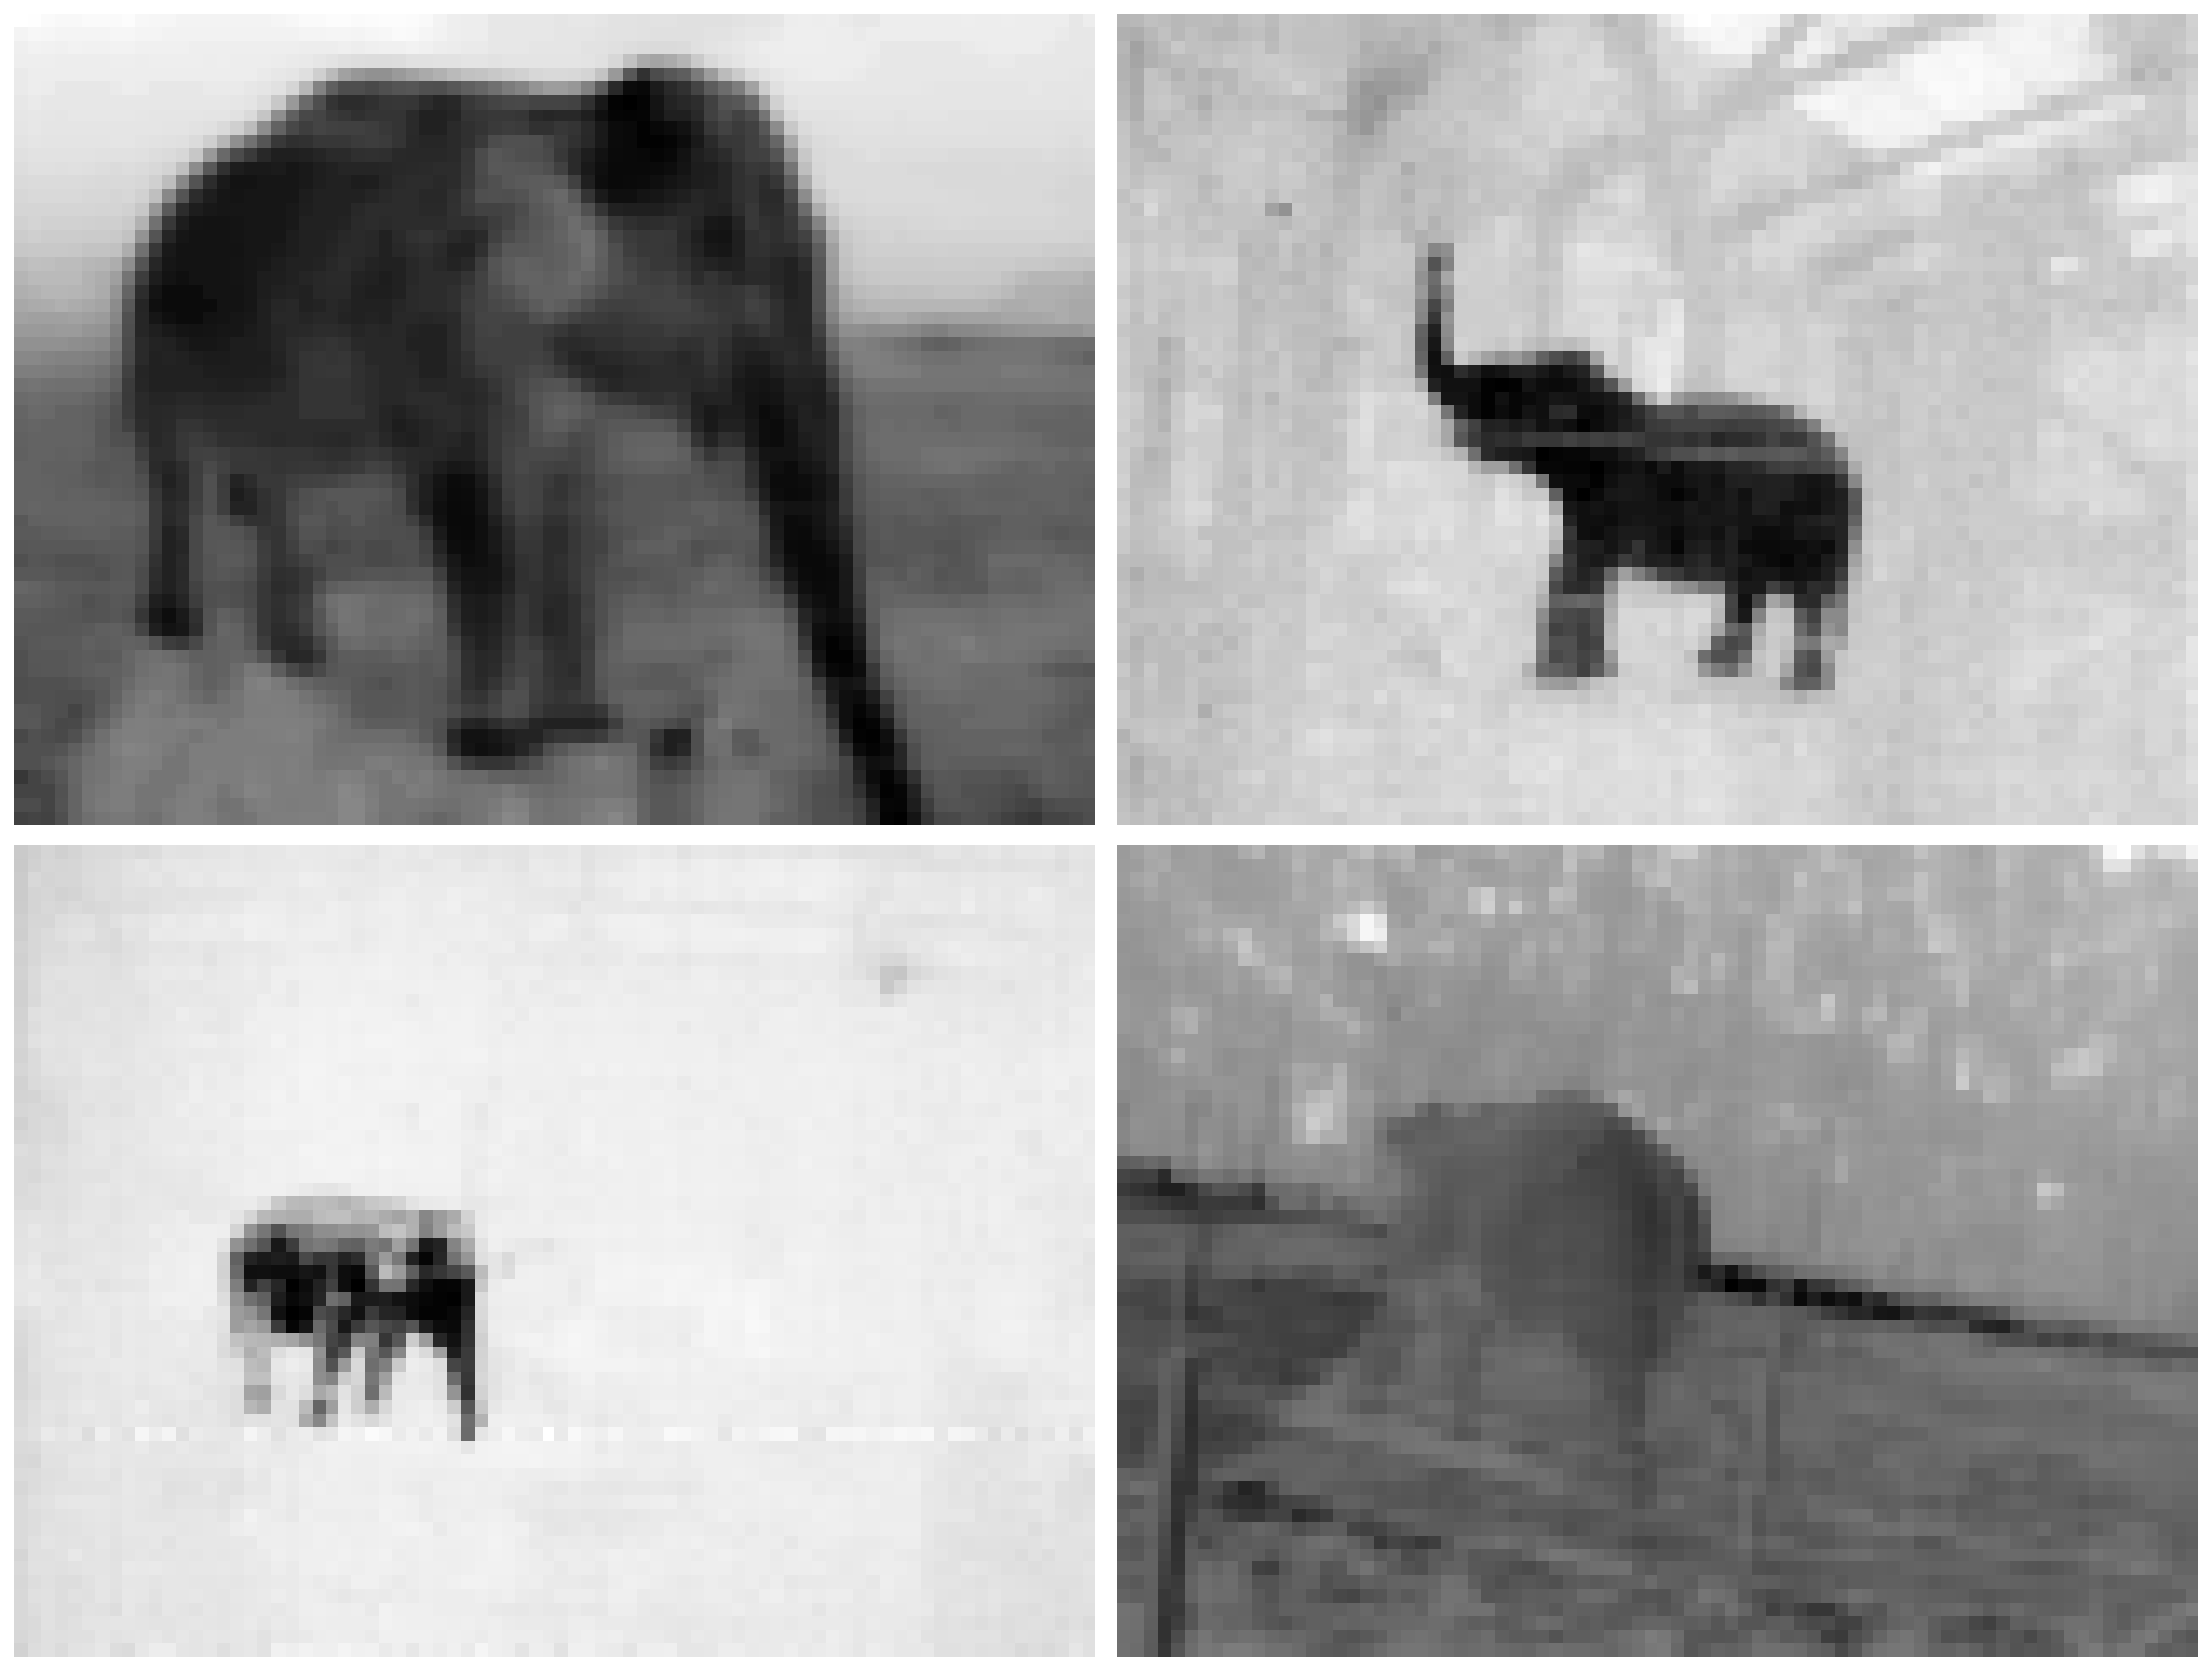
\includegraphics{four_elephants.pdf}}
    \caption{Thermal images of elephants from dataset.}
    \label{four_elephants}
\end{figure}

Thermal image dataset was given to us in form of a Google Drive folder, which we downloaded to our computer.
After examining the folder, we came to several conclusions.

Firstly, we saw that the primary focus of Arribada team was to build an object localization model, not an image classification model.
In object localization neural network draws bounding boxes around objects that it recognizes and assigns them labels, while image classification model only labels the image as whole.
Object localization produces a bigger and more complex model then image classification and it is unsuitable for running on a microcontroller.
All major work that was done by Arribada team was contained in one folder where each image had accompanying text file of the same name.
Text files were produced by a DeepLabel software, which is used for preparing images for training object localization models.
Each line in a text file described a location of the bounding box and its label.
This dataset format was not suitable for us, as many images contained more bounding boxes, which would be troublesome to sort into a distinct label.
We later saw that there were few folder with names such as "Human", "Single Elephant", "Multiple Separate Elephants", "Multiple obstructing Elephants", "Cows", "Goats" and so on, which contained sorted images that we could use.
All folders with elephant pictures we merged into one folder, as we did not care if model can differentiate how many elephants are on a taken image, we only wanted to know if there are any elephants on it or not.

Secondly, we found out that all images were documented in a large Excel database.
For each image there was a row in a database that connected image file name with information where image was taken and with what sensor.
This enabled us to generate a graph seen on Figure \ref{nested_donut1}.
We used a total of 13667 images from thermal image dataset, almost 88 \% of them were made in Whipsnade Zoo, the rest of them were made in Assam.
All images from Assam were made with FLIR Lepton 2.5, while both cameras were used in Whipsnade zoo, however more photos were made with 2.5 version of the thermal camera.

\begin{figure}[ht]
    \centering
    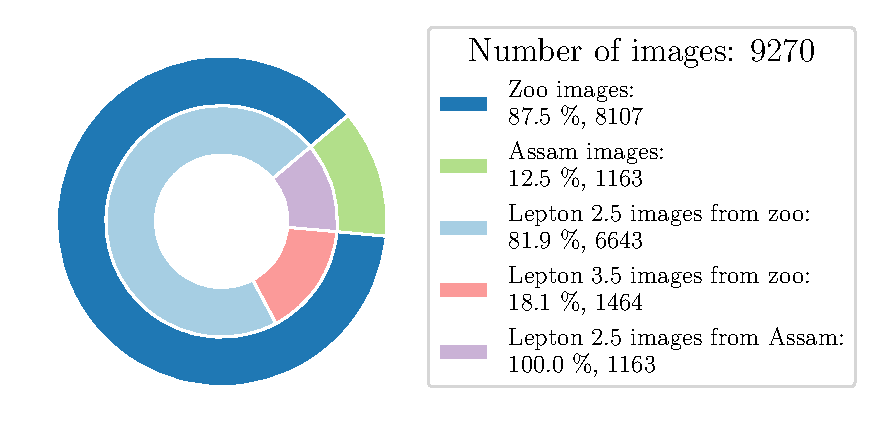
\includegraphics{nested_donut1.pdf} 
    \caption{Distribution of used images depending on image location and type of sensor.}
    \label{nested_donut1}
\end{figure}

Thirdly, after manually inspecting the folder with goat images we saw that it mostly contained images of a goat herd, standing around a single elephant.
This folder was usable only for object localization ML models, where each goat could be tagged with a bounding box. 
In case of an image classification model, this sort of training data is not desirable, as it would be too similar to another separate class, in our case elephant class.
We therefore dropped goat images out of our training data entirely.

Additionally, we realised that there was a large class imbalance, as seen on Figure \ref{nested_donut2} in favor to elephant class.
Number of elephant images was more than 4 times larger from the number of images of the all other classes combined.
This issue was solved with acquiring more images of the minority class, oversampling the minority class and/or undersampling the majority class and additionally augmenting images in preparation phase.

\begin{figure}[ht]
    \centering
    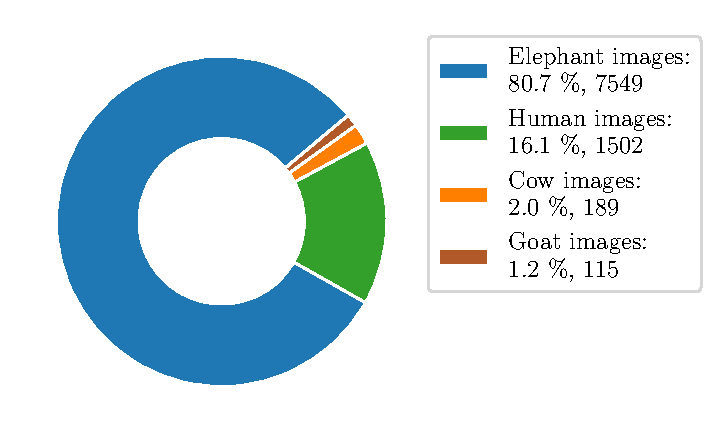
\includegraphics{nested_donut2.pdf} 
    \caption{Class distribution of thermal images.}
    \label{nested_donut2}
\end{figure}

\subsection{ Gathering thermal images}

As the amount of cow images was low compared to human and elephant classes and because we also did not had any images that would fit into nature/random class, we decided to gather them ourselves.
We wanted to do this as quickly and efficiently as possible so we build a prototype camera made out of FLIR Lepton 2.5 breakout board, Raspberry Pi Zero and power bank.
We used an open source library \cite{flir_github} for FLIR Lepton module which used a simple C program to take a single image with a thermal camera and save it to a Raspberry Pi.
Image of the setup can be seen on Figure \ref{cow_camera}.

\begin{figure}[ht]
    \centering
    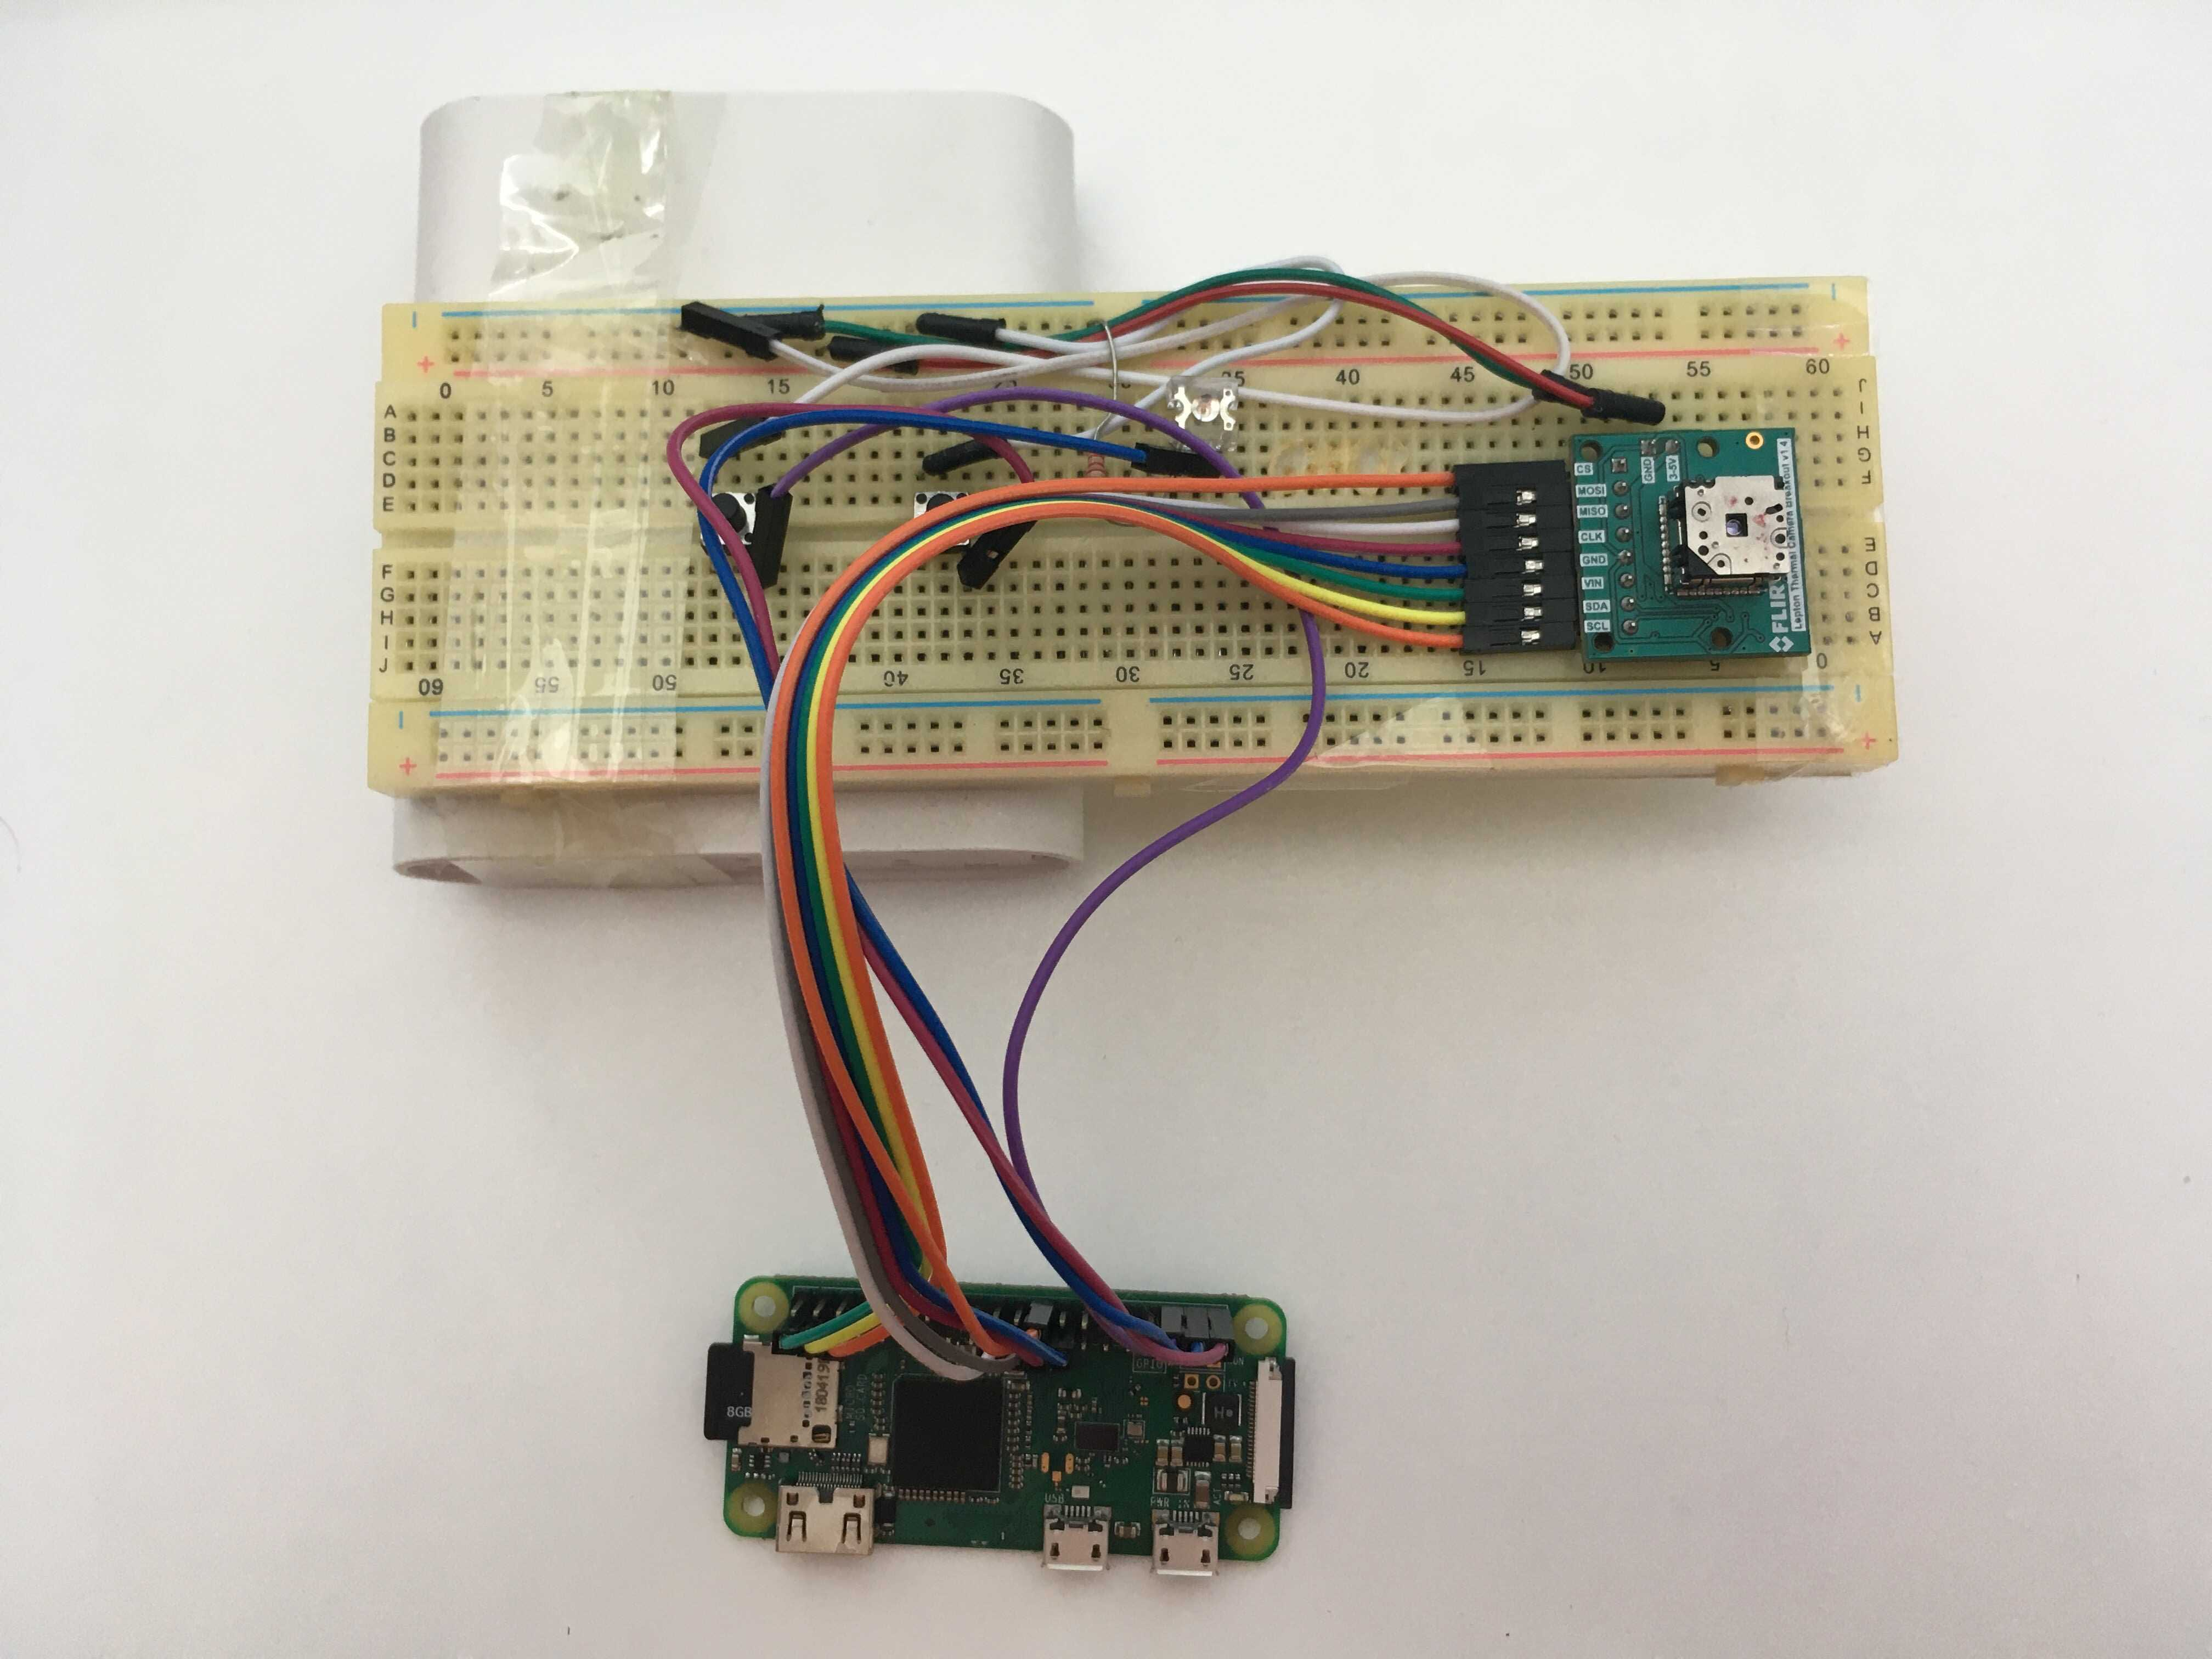
\includegraphics[width=1.0\linewidth]{cow_camera.jpg} 
    \caption{Camera setup used for taking thermal images with FLIR Lepton 2.5.}
    \label{cow_camera}
\end{figure}

We wrote a simple Python script which executed C program every time we pressed the trigger push-button.
Additional shutdown button was added to call the Raspberry Pi shutdown routine, as forcibly removing power from it would corrupt freshly taken thermal images on the Raspberry Pi's SD card.

With this setup we made 365 images of cows in varying conditions, 308 images of nature and 124 images of a human that were made on the go.
We then manually sorted images into appropriate folders and added them to the dataset.


\section{ Development environment}

All of the work around image preparation and ML model creation was done using Amazon's Elastic Compute Cloud web service.
Elastic Compute Cloud or EC2 enables users to create an instance of a server in a cloud with specified amount of processing power and memory.
Some instances come with dedicated software modules and dedicated graphics cards for extra boost in performance.

As we did not had powerful hardware at our disposal, we created an instance of Linux server that came with TensorFlow, Numpy and other libraries pre-installed.
We interacted with the server's command line through SSH protocol.

Because TensorFlow has a Python API, we needed to write some Python code.
Instead of writing Python scripts and executing them through command line, we used Juptyer Notebook. 
Juptyer Notebook is a web-based application that can run programs that are a mix of code, explanatory text and computer output.
Users can divide code into segments, which can be executed separately, visual output from modules such as Matplotlib is also supported.
Separate phases of model creation can also be split in several different files to improve readability and reuse.
To setup Juptyer Notebook on our cloud instance, we only had to install it with package manager, run it and expose default 8888 port that it uses on the Amazon's server configuration site to the public.
We could then access web service simply through web browser by writing the IP address of the server, followed by the 8888 port.


\section{ Image preparation}

Image preparation phase is a pipeline process that differs from project to project.
Our process can be seen on Figure \ref{image_preparation}.

\begin{figure}[ht]
    \centering
    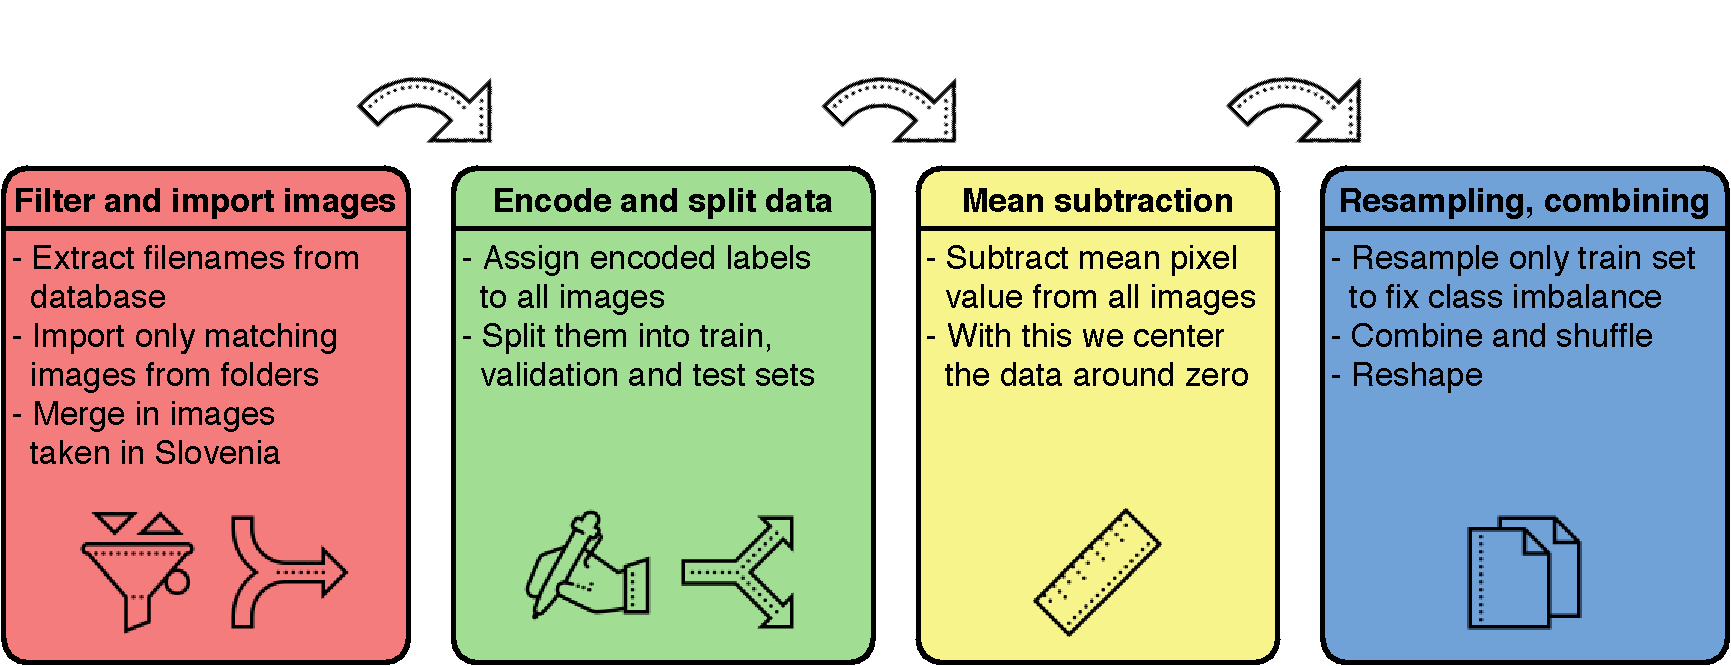
\includegraphics[width=1.0\linewidth]{image_preparation.pdf} 
    \caption{Image preparation pipeline that was used. Icons source: www.icons8.com.}
    \label{image_preparation}
\end{figure}

At the start of the process we compared filenames of each separate folder to the list of filenames found in Excel database.
We imported only the images found in both sources, as lists were not identical and we wanted to keep track of different metadata information.
As some images were made with two different FLIR Lepton camera with different resolutions (60 x 80 and 120 x 160), we just downscaled higher resolution directly in the importing process.
After this we simply added images that were taken by us in Slovenia.
At this point we had four separate Numpy arrays, one for every class, with 3 dimensions: first dimension was a number of different images in that class, second and third dimensions stored image's pixel values (60 and 80 pixels respectively).

Next step was assigning labels to every image.
As the output of NNs are numbers, we can not just assign labels in strings format to data.
Instead we assigned every image a single number that represented that class, 0 for elephant, 1 for human, 2 for cow and 3 for nature/random class.
We shuffled images inside of each class and then split them into training, validation and test sets.
At end of this step we had 4 different Python dictionaries for each class.
Each dictionary had 3 key-value pairs for every training, validation and test set, which held image data and encoded labels.

We next applied simplest form of normalization to all images, a mean subtraction.
We calculated a two dimensional matrix that held mean values of pixels averaged over the whole training set, which we subtracted from all images, essentially zero centering the data.
This is a common preprocessing step in every ML image pipeline, which is usually combined with standardization\cite{cs231n}.
Standardization scales the whole range of input pixel values into -1 and 1 interval.
This is only needed if different input values have widely different ranges\cite{cs231n}.
Because images that were created with FLIR camera were all 8-bit encoded, therefore same range, this was not needed.

In the end we had to fix our imbalance problem.
We achieved this by resampling the human, cow and nature/random classes.
Human class was resampled three times, while both cow and nature/random classes were resampled six times.
Figure \ref{resampled} shows distribution of training images before and after resampling.

\begin{figure}[ht] 
    \begin{subfigure}[b]{1\textwidth}
        \centering
        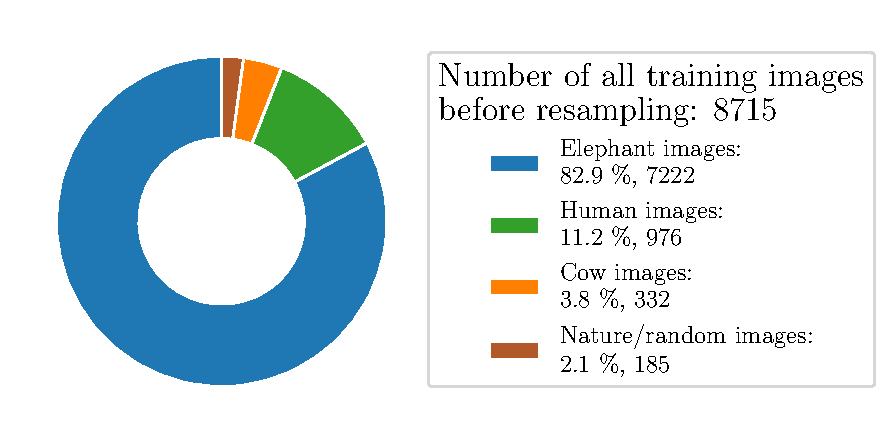
\includegraphics[width=1.0\linewidth]{nested_donut3.pdf} 
    \end{subfigure}
    \unskip\ \hrule\ 
    \begin{subfigure}[b]{1\textwidth}
        \centering
        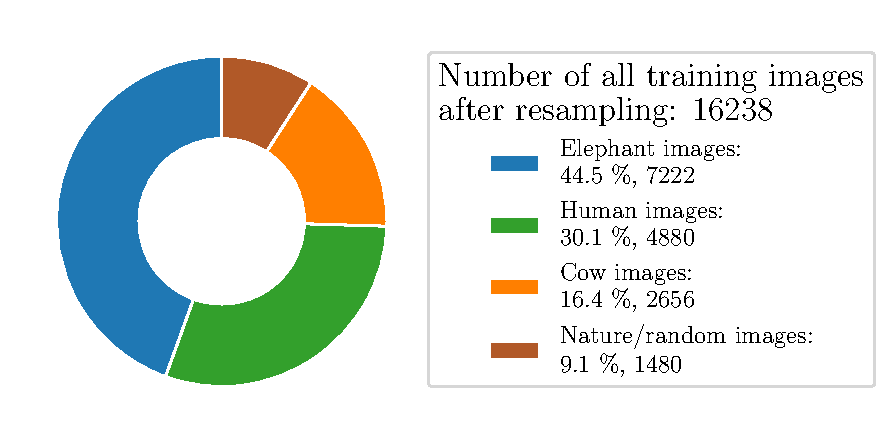
\includegraphics[width=1.0\linewidth]{nested_donut4.pdf} 
    \end{subfigure}
    
    \caption{ Distribution of training images before and after resampling.}
    \label{resampled}
\end{figure}

We only resampled training sets, not validation or test sets.
If we resampled everything, model would be seeing same image several times during testing, thus reporting incorrect accuracy in validation and test phase.

After resampling we merged and shuffled all data and reshaped it with Numpy from three dimensions to four, so it was ready for model training.


\section{ Model creation and training}

For creating CNN models we used Keras Sequential API. 
With it programmer creates a model and adds layers one by one.
When adding layers we are only specifying what type of layer we went, size of it and layer specific features. 
We do not need to keep track of any connections between or in layers, this is done automatically by Keras.
Specific architecture of models that we created can be seen in section TODO ADD REFERENCE, however in Figure \ref{} we can see Keras code and summary of the model that it created.

\definecolor{codegreen}{rgb}{0,0.6,0}
\definecolor{codegray}{rgb}{0.5,0.5,0.5}
\definecolor{codepurple}{rgb}{0.58,0,0.82}
\definecolor{backcolour}{rgb}{0.95,0.95,0.92}

\lstdefinestyle{mystyle}{
    backgroundcolor=\color{backcolour},   
    commentstyle=\color{codegreen},
    keywordstyle=\color{magenta},
    numberstyle=\tiny\color{codegray},
    stringstyle=\color{codepurple},
    basicstyle=\linespread{0.9}\ttfamily\footnotesize,
    breakatwhitespace=false,         
    breaklines=true,                 
    captionpos=b,                    
    keepspaces=true,                 
    numbers=left,                    
    numbersep=5pt,                  
    showspaces=false,                
    showstringspaces=false,
    showtabs=false,                  
    tabsize=2
}

\lstset{style=mystyle}

\begin{lstlisting}[language=Python]
model = models.Sequential()
model.add(layers.Conv2D(32, (3, 3), activation='relu', 
        input_shape=(60,80, 1)))
model.add(layers.MaxPooling2D((2, 2)))
model.add(layers.Conv2D(64, (3, 3), activation='relu'))
model.add(layers.MaxPooling2D((2, 2)))
model.add(layers.Conv2D(64, (3, 3), activation='relu'))
model.add(layers.Flatten())
model.add(layers.Dense(64, activation='relu'))
model.add(layers.Dense(4))

# Show the model's architecture
model.summary()

Model: "sequential"
_________________________________________________________________
Layer (type)                 Output Shape              Param #   
=================================================================
conv2d (Conv2D)              (None, 58, 78, 32)        320       
_________________________________________________________________
max_pooling2d (MaxPooling2D) (None, 29, 39, 32)        0         
_________________________________________________________________
conv2d_1 (Conv2D)            (None, 27, 37, 64)        18496     
_________________________________________________________________
max_pooling2d_1 (MaxPooling2 (None, 13, 18, 64)        0         
_________________________________________________________________
conv2d_2 (Conv2D)            (None, 11, 16, 64)        36928     
_________________________________________________________________
flatten (Flatten)            (None, 11264)             0         
_________________________________________________________________
dense (Dense)                (None, 64)                720960    
_________________________________________________________________
dense_1 (Dense)              (None, 4)                 260       
=================================================================
Total params: 776,964
Trainable params: 776,964
Non-trainable params: 0
_________________________________________________________________
\end{lstlisting}


\section{ Model optimizations}

For model optimization phase we wrote a Python script that took model in .h5 format and converted it into four differently optimized tflite models:
\begin{itemize}
    \item \textbf{Non-quantized tflite model,} no quantization, just basic conversion from .h5 to .tflite format is done.
    \item \textbf{float16 model,} weights are quantized from 32-bit to 16-bit floating-point values. Model size is split in half and accuracy decrease is minimal, but there is no boost in execution speed.
    \item \textbf{dynamic model,} weights are quantized as 8-bit values, but operations are still done in a floating-point math. Models are 4 times smaller and execution speed is faster when compared to float16 optimization but slower from full integer optimization.
    \item \textbf{Full integer model,} weights, biases and math operations are quantized, execution speed is increased. It requires representative dataset at time of optimization.
\end{itemize}

Full integer model is an ideal choice for running models on microcontrollers, however it should be noted that not all operations have full integer math implementations in TFLite Micro.
Script also uses tool xxd to create .c and .h files of models in c array format, for later inference on microcontroller.

\section{ Edge Impulse (SHOULD this be here like that, how should i go about this)}
